\begin{thema}{Β}
Δίνονται οι γραφικές παραστάσεις των $f$ (μπλε) και $g$ (κόκκινη) στο $[0, 5]$. Η $f$ είναι τμηματικά γραμμική: $f(0)=1, f(2)=3, f(4)=1, f(5)=2$. Η $g$ ορίζεται: $g(0)=0, g(1)=2, g(2)=4, g(3)=3, g(5)=1$.

\begin{center}
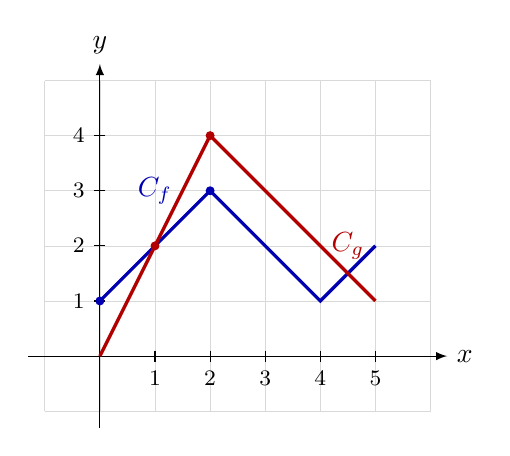
\begin{tikzpicture}[scale=0.7]
  \draw[help lines, gray!30] (-1,-1) grid (6,5);
  \draw[-latex] (-1.3,0) -- (6.3,0) node[right] {$x$};
  \draw[-latex] (0,-1.3) -- (0,5.3) node[above] {$y$};
  \foreach \x in {1,2,3,4,5}
    \draw (\x,0.1) -- (\x,-0.1) node[below,font=\footnotesize] {$\x$};
  \foreach \y in {1,2,3,4}
    \draw (0.1,\y) -- (-0.1,\y) node[left,font=\footnotesize] {$\y$};
  % f
  \draw[very thick, blue!70!black] (0,1) -- (2,3) -- (4,1) -- (5,2);
  \node[blue!70!black] at (1,3) {$C_f$};
  % g
  \draw[very thick, red!70!black] (0,0) -- (1,2) -- (2,4) -- (3,3) -- (5,1);
  \node[red!70!black] at (4.5,2) {$C_g$};
  % key points
  \filldraw[blue!70!black] (0,1) circle (2pt);
  \filldraw[blue!70!black] (2,3) circle (2pt);
  \filldraw[red!70!black] (1,2) circle (2pt);
  \filldraw[red!70!black] (2,4) circle (2pt);
\end{tikzpicture}
\end{center}

\begin{erwthma}
  \item Να υπολογίσετε $(f \circ g)(1)$, $(g \circ f)(2)$ και $(f \circ f)(0)$.
  \item Να βρείτε $(f+g)(2)$, $(f \cdot g)(0)$ και $\frac{f}{g}(3)$.
  \item Η σύνθεση $(g \circ f)(x)$ ορίζεται στο $x = 4$; Υπολογίστε, αν ναι.
  \item Λύστε γραφικά την εξίσωση $f(x) = g(x)$.
\end{erwthma}
\end{thema}
